\documentclass[12pt,a4paper]{article}
\usepackage[utf8]{inputenc}
\usepackage[T1]{fontenc}
\date{} 
\usepackage[spanish]{babel}
\usepackage{amsmath}
\usepackage{amsfonts}
\usepackage{amssymb}
\usepackage{graphicx}
\usepackage{mathpazo} % Palatino font
\usepackage[left=2.50cm, right=2.50cm, top=1.50cm, bottom=1.50cm]{geometry}
\author{Caamiña, Daniela \and Yapura, Cristian}
\title{Trabajo final \\Automatización industrial}
\graphicspath{ {images/} }

	
\begin{document}
	\begin{titlepage} %Carátula 			
		\newcommand{\HRule}{\rule{\linewidth}{0.5mm}} 
		\center % Centre everything on the page		
		\textsc{\LARGE Universidad Nacional de la Patagonia San Juan Bosco}\\[1.5cm]
		\textsc{\Large Automatización Industrial}\\[0.5cm]
		\textsc{\large Trabajo Final}\\[0.5cm] 
		\HRule\\[0.4cm]
		\huge\bfseries{Banco de pruebas para motor trifásico}\\[0.2cm] 
		\HRule\\[1.5cm]
			\begin{minipage}{0.4\textwidth}
				\begin{flushleft}
					\large
					\textit{Alumnos}\\
					\textsc{Caamiña,} Daniela \\
					\textsc{Yapura,} Cristian  
				\end{flushleft}
			\end{minipage}
			\begin{minipage}{0.4\textwidth}
				\begin{flushright}
					\large
					\textit{Docentes}\\
					Ing. \textsc{Lorenc,} Marcelo \\
					Dr. \textsc{Peña,} Ramiro  
				\end{flushright}
			\end{minipage}
		\vfill\vfill\vfill 
		\large{Junio 2020} 
		\vfill\vfill
		\includegraphics[width=0.2\textwidth]{unpsjb.png}\\[1cm] 
		\vfill 
	\end{titlepage}
	
\tableofcontents
\newpage

\listoffigures
\newpage	
	
	\part{Introducción}
	\newpage

	
	\part{Objetivo}
	Realizar un banco de pruebas y una interfaz gráfica para un motor trifásico conectado a un variador de velocidad a través de un PLC.\\
	VER EJEMPLOS QUE SIGUEN PARA USAR EN OBJETIVOS O EN CONCLUSIONES\\
	.-Comprender los   métodos de   conexionado   entre   PLC   y   variador   de frecuencia..\\-Comparar   los   métodos   de   conexionado   en   función   delnúmero   de conductores a utilizar y del tiempo de respuesta..\\-Diferenciar entre la transferencia de datos de control (PLC-Variador) y datos de supervisión (Variador -PLC).

	\newpage
	\part{Motor}
	\section{Especificaciones}
	El motor (Figura \ref{fig:motor}) asincrónico que se utiliza es de la marca \textbf{Altium} perteneciente a la firma \textbf{Schneider Electric}. Las especificaciones se muestran a continuación
	\paragraph*{Altium Eff2}
	\begin{itemize}
		\item 	Tipo: TE2A90SP2
		\item   Tensión nominal: 220/380 V
		\item 	Corriente nominal: 5.97 A 
		\item	Frecuencia nominal:  50 Hz.
		\item 	Potencia: 1.5kW / 2 HP
		\item 	Fases: 3
		\item   Factor de Potencia: 0.84
	\end{itemize}
	
	\begin{figure}[h!]
		\centering
		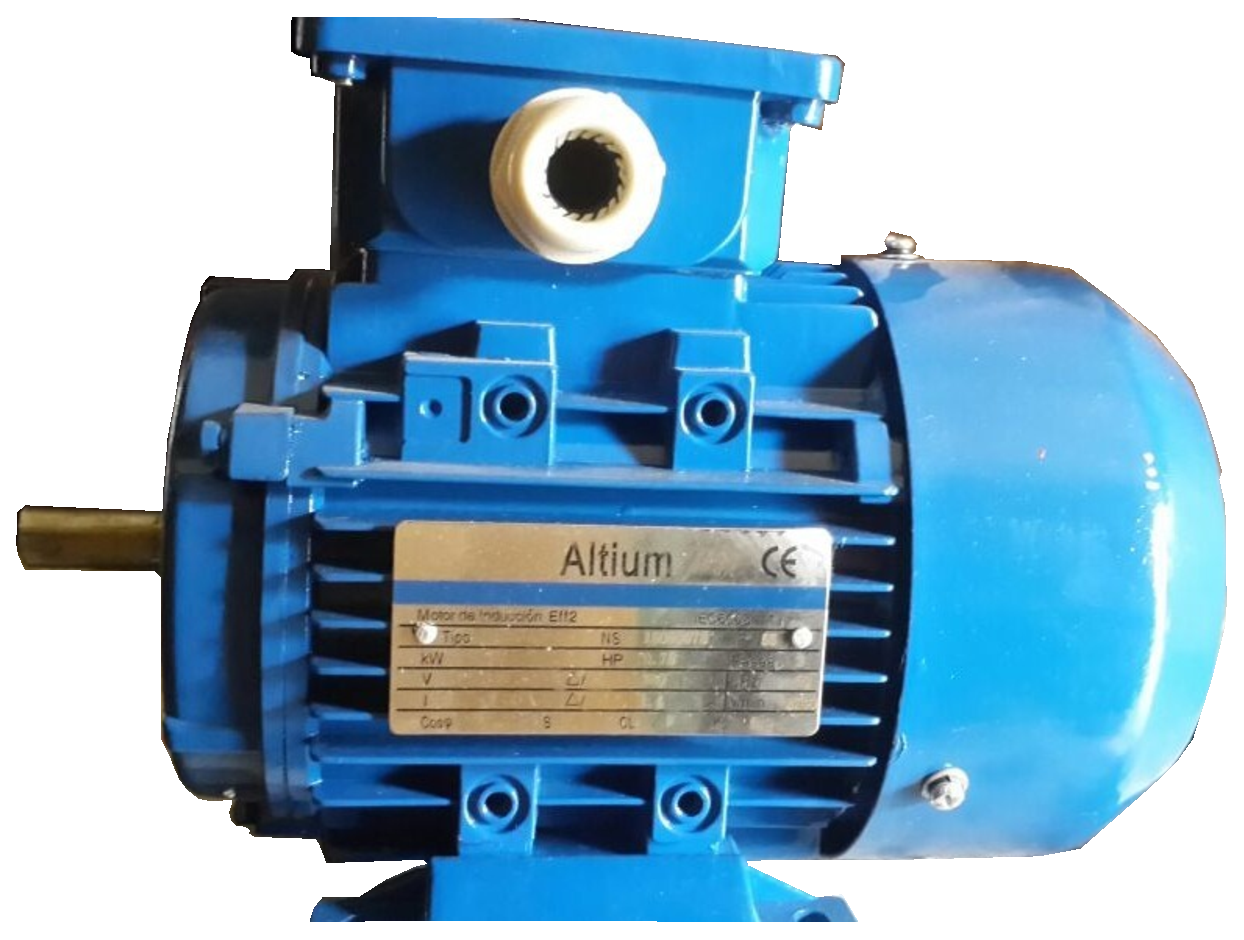
\includegraphics[scale=0.4]{motor.eps}
		\caption{Motor Altium}
		\label{fig:motor}
	\end{figure}
	
	
	\newpage
	\part{Variador de velocidad}
		\section{Especificaciones}
		El variador de velocidad que se utilizó pertenece a la marca \textbf{Schneider Electric} (Figura \ref{fig:variador}) que posee las siguientes características.
		\paragraph*{Altivar 312}
		\begin{itemize}
			\item 	Modelo: ATV312HU15N4
			\item   Tensión: 380-500 V
			\item 	Frecuencia: 50/60 Hz
			\item 	Potencia: 1.5kW / 2 HP
			\item 	Fases: 3
		\end{itemize}

		\begin{figure}[h!]
			\centering
			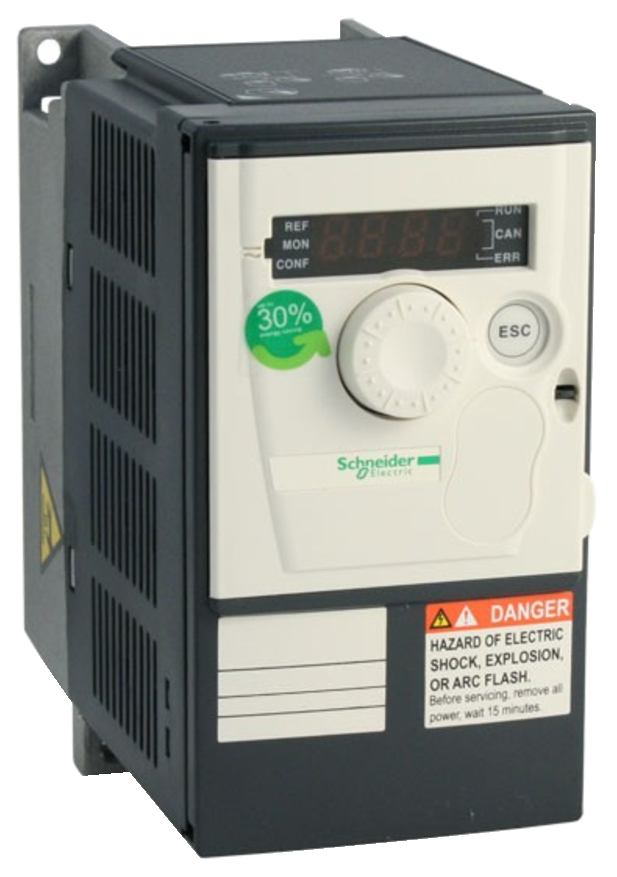
\includegraphics[scale=0.4]{variador.eps}
			\caption{Variador de velocidad Altivar 312}
			\label{fig:variador}
		\end{figure}

		\section{Restauración de fábrica}
		Para modificar el variador desde el dispositivo se sabe que cada aceptación del parámetro o ingreso al menú se realiza presionando el botón central blanco y para buscar estos es necesario girar la misma. Para salir, tan solo presionar botón \textsl{ESC} tantas veces como sea necesarias. \\
			\begin{figure}[h!]
			\centering
			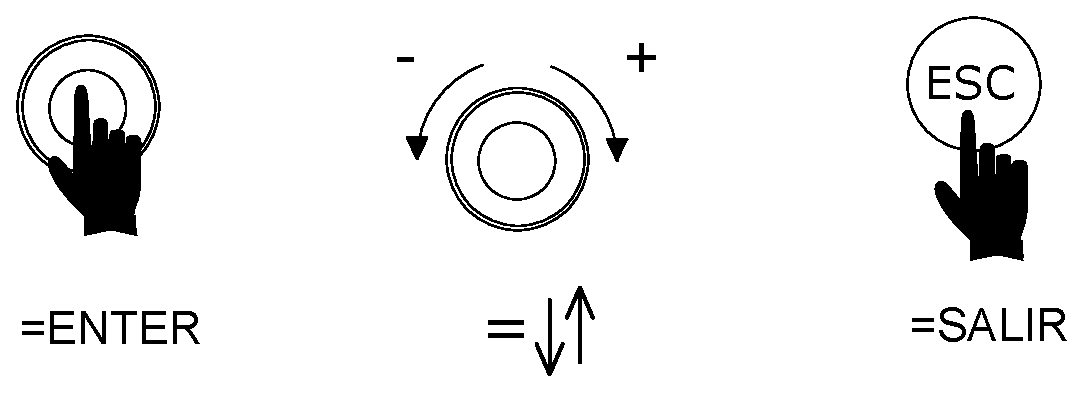
\includegraphics[scale=0.5]{ver2.eps}
			\caption{Comandos básicos del panel}
			%\label{fig:frente}
			\end{figure}
	
	Para comenzar a realizar la configuración del variador de velocidad primero se procede a restaurarlo de fábrica.
			
			\begin{figure}[h!]
			\centering
			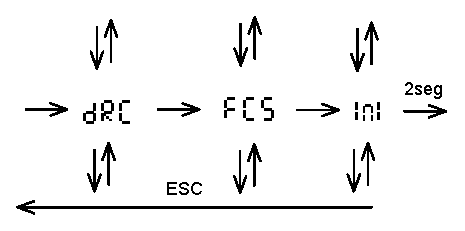
\includegraphics[scale=1]{ver1.eps}
			\caption{Restauración de fábrica}
			%\label{fig:BME280}
			\end{figure}

	\section{Configuración de parámetros primarios}
	El paso siguiente será la configuración de los parámetros del motor que se utilizará: \textsl{Frecuencia estándar del motor; tensión nominal del motor, frecuencia nominal, corriente nominal, factor de potencia}\\
	\textbf{usar las imagenes en autocad}
	
		
\newpage
	
	\part{PLC}
	
	Que modulos tiene PLC M340????
	\section{Especificaciones}
	\section{Comunicación}
	\begin{figure}[htb]
		\centering
		\includegraphics[scale=0.7]{comu.png}
		%\caption{Placa BME280}
		%\label{fig:BME280}
	\end{figure}
\newpage
	\part{Banco de pruebas}
		\section{Construcción}
		\section{Elementos}
		Se decidió que el banco de pruebas cuente con los siguientes elementos:
		\begin{itemize}
			\item interruptor
			\item botón de marcha/ parada
			\item botón parada de emergencia
			\item señalización lumínica
			\item freno para generar perturbaciones 
			\item riel para colocar un nuevo motor que actuará como carga
		\end{itemize}
		\section{Presupuesto--Valor--Costo a tal día}
	\newpage
	
	\part{Comunicación}
	
	El   variador   también   se   puede   controlar   en   modo   remoto.   Es   adecuado   paraaplicaciones en   los   que   los   cambios   de   variables   del   variadorse   realizan frecuentemente  durante  el proceso.  Dichos  cambios  pueden  realizarse  por  parte  del propio  operario  (mediante  potenciómetros,  interruptores,  selectores  rotativos  o  BCD, etc.).  Sin  embargo,  la  situación  más  común  es  que  los  parámetros  del  variador  los establezca  el  equipo  de  control  y  supervisión  del  proceso,  al  que  está  conectado  el variadorde  frecuencia: reguladores  de  tensión  y/o  corriente,  finales  de  carrera, pantallas de operador, etc., o incluso un ordenador personal y/o PLC. Para  el  casode  estos  controles  remotos,  la  comunicación  se  puede  realizarde  dos modos:\\Mediante un  número  determinado  de  conductores,  que  depende  de  los elementos que se tengan conectados al variador de frecuencia, por el que se transmiten señales digitales (finalesde carrera, interruptores, salidas digitales de un PLC), o analógicas (potenciómetro, salida analógica de un PLC):\\Mediante un bus de comunicaciones industriales (de 2 o 4 hilos), sobre el que se transmiten   mensajes   de   ajuste   de   parámetros   siguiendo   un   protocolo preestablecido (Modbus, CanBus, ProfiBus, EtherCat, etc.).Con 2  conductores la  comunicación  se  hace  más  lenta(modo  semidúplex),  pero  lógicamente representa un menor coste.
	
	
	

	\section{CANopen}
	\section{Modbus}
	
	\section {HMI}
	Se realizó una interfaz humana maquina con los siguientes elementos:
		\begin{itemize}
			\item boton de start(acá o en el tablero???)
			\item varias velocidades configuradas previamente
			\item inversión y señalización del mismo
			\item torque???
		\end{itemize}
		\begin{figure}[htb]
			\centering
			\includegraphics{HMIej.png}
			%\caption{Placa BME280}
			%\label{fig:BME280}
		\end{figure}
 	\part{Conclusiones}
 		Realizar un banco de pruebaSSSSsssssssssSSSSs de un motor trifásico conectado a un variador de velocidad a través de un PLC generando una interfaz para el usuario.\\
 	VER EJEMPLOS QUE SIGUEN PARA USAR EN OBJETIVOS O EN CONCLUSIONES\\
 	.-Comprenderlos   métodos de   conexionado   entre   PLC   y   variador   de frecuencia..\\-Comparar   los   métodos   de   conexionado   en   función   delnúmero   de conductores a utilizar y del tiempo de respuesta..\\-Diferenciar entre la transferencia de datos de control (PLC-Variador) y datos de supervisión (Variador -PLC).
 	\part{Anexos}

	
\end{document}